\documentclass[a4paper,12pt]{report}
\usepackage{graphicx}
\graphicspath{{picaa/}}
\usepackage{listings}
\usepackage{amsmath}
\usepackage[T2A]{fontenc}
\usepackage[utf8]{inputenc}
\usepackage[english,russian]{babel}
\usepackage{pgfplots} 

\usepackage{geometry}
\geometry{left=2cm}
\geometry{right=1.5cm}
\geometry{top=1cm}
\geometry{bottom=2cm}
\lstset{language = C++,
	keywordstyle = \color{orange},
	stringstyle = \color{green},
	commentstyle = \color{red},
	columns = fullflexible
}

\begin{document}

    \begin{titlepage}

        \begin{center}
            \large
            \textbf{Государственное образовательное учреждение высшего профессионального образования\\
            “Московский государственный технический университет имени Н.Э.Баумана”\\}
            
\includegraphics{bmstu-logo.png}
			\vspace{1cm}
            
            \textsc{Дисциплина: Анализ алгоритмов}
            \vspace{0.5cm}
                
            \textsc{Лабораторная работа №4}
            \vspace{1cm}
            
            {\LARGE \textbf{Исследование параллельных вычислений на основе параллельного алгоритма Винограда}}
            \vspace{3cm}
                    
            \begin{flushright}
            	Студент группы ИУ7-55Б,\\   
            	Руднев К. К.,\\
            	\vspace{0.5cm}
            	Преподаватель,\\
            	Волкова Л. Л.,\\
            	Строганов Ю. В.
            	
            \end{flushright}
            \vfill
            
            2019 г.
            
            \end{center}

    \end{titlepage}

	\setcounter{page}{2}
	\tableofcontents
	\chapter*{Введение}

		Цель работы: изучение возможности параллельных вычислений и использование такого подхода на практике, а также реализация параллельного алгоритма Винограда умножения матриц. 
		В данной лабораторной работе рассматривается алгоритм Винограда и параллельный алгоритм Винограда.
		
		Задачи:
		\begin{itemize}
			\item сравнить зависимость времени от числа параллельных потоков и размера матриц;
			\item разработать алгоритм для умножения матриц алгоритмом Винограда последовательно;
			\item разработать алгоритм для умножения матриц алгоритмом Винограда параллельно;
			\item провести сравнение стандартного и однопоточного параллельного алгоритмов.
		\end{itemize}

    \label{sec:intro}

    \newpage

    \chapter{Аналитическая часть}
        \label{sec:analitic_part}

        	В рамках раздела будет дано аналитическое описание алгоритма для умножения матриц по Винограду, а также идеи его распаралелливания.

	\section{Описание алгоритмов}
        
        	Пусть даны две прямоугольные матрицы A[MxQ] и B[QxN]:\\
        	A = $\begin{bmatrix}
        		a_{11}& a_{12}& ...& a_{1Q}\\
        		a_{21}& a_{22}& ...& a_{1Q}\\
        		.& .& .& .\\
        		.& .& .& .\\
        		.& .& .& .\\
        		a_{M1}& a_{M2}& ...& a_{MQ}\\
        	\end{bmatrix}$, B = $\begin{bmatrix}
        		b_{11}& b_{12}& ...& b_{1N}\\
        		b_{21}& b_{22}& ...& b_{1N}\\
        		.& .& .& .\\
        		.& .& .& .\\
        		.& .& .& .\\
        		b_{Q1}& b_{Q2}& ...& b_{QN}\\
        	\end{bmatrix}$ .
        	
        	\vspace{0.3cm}
        	Тогда матрица C[MxN]:\\
        	C = $\begin{bmatrix}
        		c_{11}& c_{12}& ...& c_{1N}\\
        		c_{21}& c_{22}& ...& c_{1N}\\
        		.& .& .& .\\
        		.& .& .& .\\
        		.& .& .& .\\
        		c_{M1}& c_{M2}& ...& c_{MN}\\
        	\end{bmatrix}$, в которой:\\
        	
        	\vspace{0.3cm}
        	\begin{multline}
        		\label{func:std}
        		c_{ij} = \sum\limits_{r=1}^m a_{ir}*b_{rj} \ (i=1,2,...M; j=1,2,...N).
        	\end{multline} называется их произведением \cite{Beloysov}.\\
        	
        	\vspace{0.6cm}
        	
        	\subsection{Алгоритм Винограда}
        	
        	Подход алгоритма Винограда является иллюстрацией общей методологии, начатой в 1979-х годах на основе билинейных и трилинейных форм, благодаря которым большинство усовершенствований для умножения матриц были получены \cite{Gall2012}.
        	Пусть даны две прямоугольные матрицы A[1xQ] и B[Qx1]:\\
        	U = $\begin{bmatrix}
        		u_{1}& u_{2}& ...& u_{Q}\\
        	\end{bmatrix}$, V = $\begin{bmatrix}
        		v_{1}\\
        		v_{2}\\
        		.&\\
        		.&\\
        		.&\\
        		v_{Q}\\
        	\end{bmatrix}$ .
        	
        	\vspace{0.3cm}
        	Тогда матрица C[1x1]:\\
        	\begin{multline}
        		\label{func:vinograd}
        		C_{ij} = u_{1}*v_{1}+u_{1}*v_{1}+...+u_{Q}*v_{Q} =\\ (u_{1}+v_{2})*(u_{2}+v_{1})+...+(u_{Q-2}+v_{Q-2})*(u_{Q}+v_{Q})-\\
        		u_{1}*u_{2}-u_{Q-3}*u_{Q-2}-u_{Q-1}*u_{Q}-v_{1}*v_{2}-\\
        		v_{Q-3}*v_{Q-2}-v_{Q-1}*v_{Q}
        	\end{multline}
        	
        	В случае, если матрица имеет нечетную размерность, необходимо отдельно обработать последний вектор:
        	\begin{multline}
        		\label{func:vinograd_end}
        		C_{ij} = u_{in-1}*v_{n-1j}
        	\end{multline}

	\subsection{Параллельный алгоритм Винограда}
  
    		Трудоёмкость алгоритма Винограда имеет сложность O(MNQ) для умножения матрицы MxN на матрицу NxQ. 
    		Для улучшения алгоритма имеет смысл распараллелить основную часть алгоритма с тремя вложенными циклами. 
    		Опционально можно вычислять массивы mulh и mulv на разных потоках для сокращения времени. 
    		Также опционально можно производить обработку последнего вектора в отдельном потоке. 

	\section{Параллельное программирование}

    		При использовании многопроцессорных вычислительных систем с общей памятью обычно предполагается, что имеющиеся в составе системы процессоры обладают равной производительностью, являются равноправными при доступе к общей памяти, и время дотупа к памяти является одинаковым (при одновременном доступе нескольких процесоров к одному и тому же элементу памяти очередность и синхронизация доступа обеспечивается на аппаратном уровне).
    		Многопроцессорные системы подобного типа обычно именуются симметричными мультипроцессорами (symmetric multiprocessors, SMP).
    		
    		Перечисленному выше набору предположений удовлетворяют также активно развиваемые в последнее время многоядерные процессоры, в которых каждое ядро представляет практически независимо функционирующее вычислительное устройство.
    		
    		Обычный подход при организации вычислений для многопроцессорных вычислительных систем с общей памятью - создание новых параллельных методов на основе обычных последовательных программ, в которых или автоматически компилятором, или непосредственно программистом выделяются участки независимых друг от друга вычислений.
    		Возможности автоматического анализа программ для порождения параллельных вычислений достаточно ограничены, и второй подход является преобладающим. При этом для разработки параллельных программ могут применяться как новые алгоритмические языки, ориентированные на параллельноее программирование, так и уже имеющиеся языки, расширенные некоторым набором операторов для параллельных вычислений.
    		
    		Широко используемый подход состоит и в применении тех или иных библиотек, обеспечивающих определенный программный интерфейс (application programing interface, API) для разработки параллельных программ. В рамках такого подхода наиболее известны Windows Thread API. Однако первый способ применим только для ОС семейства Microsoft Windows, а второй вариант API является достаточно трудоёмким для использования и имеет низкоуровневый характер \cite{Barkalov}.
    	
    \subsection{Организация взаимодействия параллельных потоков}
    
    		Потоки исполняются в общем адресном пространстве параллельной программы.
    		Как результат, взаимодействие параллельных потоков можно организовать через использование общих данных, являющихся доступными для всех потоков.
    		Наиболее простая ситуация состоит в использовании общих данных только для чтения. В случае же, когда общие данные могут изменяться несколькими потоками, необходимы специальные усилия для организации правильного взаимодействия.

    \section{Вывод}

    		Был рассмотрен алгоритм Винограда и возможность его оптимизации с помощью распараллеливания потоков.
    		Была рассмотрена технология параллельного программирования и организация взаимодействия параллельных потоков. 

    \newpage

   \chapter{Конструкторская часть}
        \label{sec:construct_part}

        	В рамках раздела будет представлена схема алгоритма Винограда, изображенная на рисунках \ref{ris:wino1}-\ref{ris:wino5}. Также будет объявлено решение о распараллеливании этого алгоритма. 

	\section{Разработка алгоритмов}
	
		\begin{figure}[h!]
			\centering
			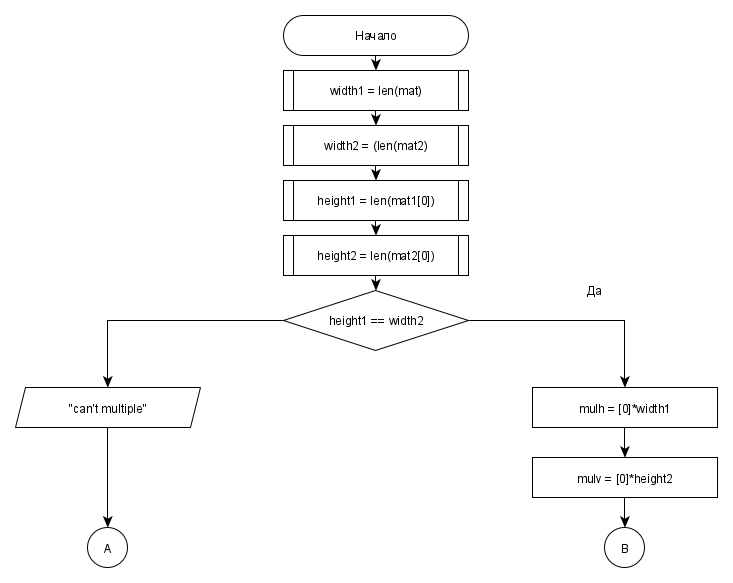
\includegraphics[width=1\linewidth]{part11.png}
			\caption{Алгоритм Винограда умножения матриц. Часть 1}
			\label{ris:wino1}
		\end{figure}
		
		\newpage
		
		\begin{figure}[h!]
			\centering
			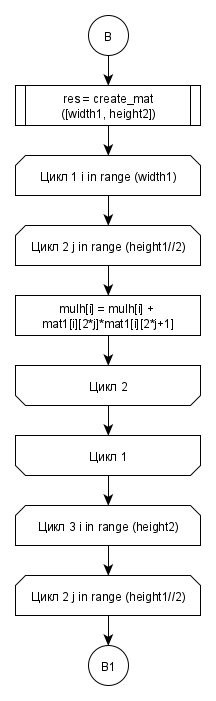
\includegraphics[width=0.4\linewidth]{part21.png}
			\caption{Алгоритм Винограда умножения матриц. Часть 2}
			\label{ris:wino2}
		\end{figure}
		
		\newpage
		
		\begin{figure}[h!]
			\centering
			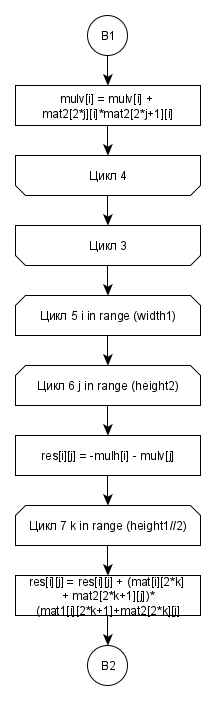
\includegraphics[width=0.4\linewidth]{part31.png}
			\caption{Алгоритм Винограда умножения матриц. Часть 3}
			\label{ris:wino3}
		\end{figure}
		
		\newpage
		
		\begin{figure}[h!]
			\centering
			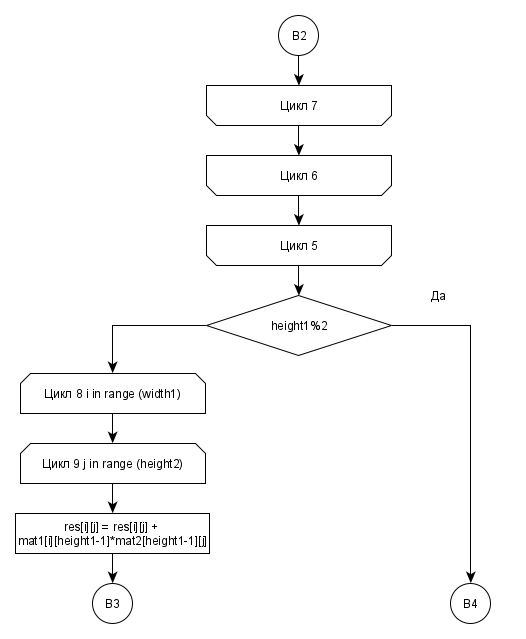
\includegraphics[width=0.8\linewidth]{part41.png}
			\caption{Алгоритм Винограда умножения матриц. Часть 4}
			\label{ris:wino4}
		\end{figure}
		
		\newpage
		
		\begin{figure}[h!]
			\centering
			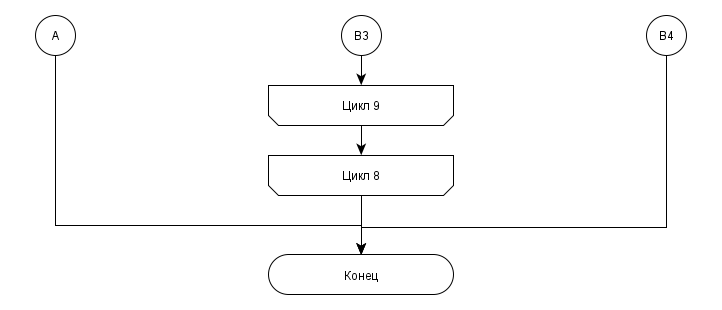
\includegraphics[width=0.8\linewidth]{part51.png}
			\caption{Алгоритм Винограда умножения матриц. Часть 5}
			\label{ris:wino5}
		\end{figure}
	
	\section{Распараллеливание алгоритма}

			Распараллеливание программы должно ускорять её выполнение.
			Это достигается за счет реализации в узким участках (например, в циклах с большим количеством независимых вычислений).
			
			В предложенном алгоритме данным участком будет являться тройной цикл поиска результата.
			Данный блок и предлагается распараллелить. На рисунках \ref{ris:wino3}-\ref{ris:wino4} этот блок представлен циклами 5-7. Также было принято решение вычислять массивы mulv и mulh в отдельных потоках.

	\section{Вывод}

			В данном разделе была рассмотрена схема алгоритма Винограда и способ её распараллеливания.

    \newpage

    \chapter{Технологическая часть}
        \label{sec:tecnologic_part}

        	Замеры времены были произведены на: Intel(R) Core(TM) i3-6006U, 2 ядра, 4 логических процессора.

	\section{Средства реализации}

			Для реализации алгоритмов использовался язык программирования C++ 11 и среда разработки QtCreator Community Edition 5.5. 
			У данного языка имеются удобные библиотеки для написания мультипоточных приложений, чего будет достаточно для реализации текущей лабораторной работы, а среда разработки имеет бесплатную коммьюнити версию и подходящий компилятор, позволяющий использовать std::threads.
			
			Замер времени реализован с помощью метода high\_resolution\_clock() класса std::chrono.
			Измеряется время исполнения кода чистого алгоритма (без учета времени на создание матриц, генерацию данных и т.п.).\\
		
	\section{Требования к программному обеспечению}

			На вход программа должна получать две матрицы, для которых вычисляется их произведение различными алгоритмами (параллельный алгоритм умножения матриц по Винограду, параллельный, но однопоточный алгоритм умножения матриц по Винограду). 
			На выход программа должна выдавать результирующую матрицу всеми алгоритмами, должна корректно обрабатывать исключительные ситуации вроде невозможности произведения данных матриц.

	\section{Листинг кода}

        	На листинге \ref{list:etc} представлены дополнительные функции и объявления, необходимые для реализации алгоритмов.
        	На листинге \ref{list:seq_wino} представлена реализация последовательного алгоритма Винограда.
        	На листинге \ref{list:par_wino} представлена реализация параллельного алгоритма Винограда.
        	
        	\begin{lstlisting}[frame = single, breaklines, caption =  Вспомогательные классы и объявления, label=list:etc]
        #include <iostream>
        #include <thread>
        #include <vector>
        #include <ctime>
        #include <memory>
        	 		
        class Imatrix
        {
        public:
        	virtual int get_rows() = 0;
        	virtual int get_cols() = 0;
        	virtual std::vector<std::vector<int>> get_mat() = 0;
        };
        		
        class matrix:Imatrix
        {
        private:
        	std::vector<std::vector<int>> mat;
        	int rows;
        	int cols;
        		
        public:
        	matrix():
        	rows(0), cols(0)
        	{}
        		
        	matrix(int n, int m):
        	rows(n), cols(m)
        	{
        		std::vector<std::vector<int>> tmp;
        		srand(time(0));
        		for (int i = 0; i < n; ++i)
        		{
        			std::vector<int> row;
        			for (int j = 0; j < m; ++j)
        				row.push_back(rand() % 10 + 1);
        			tmp.push_back(row);
        		}
        		mat = tmp;
        	}
        		
        	matrix(matrix *m1)
        	{
        		if (this != m1)
        		{
        			mat = m1->get_mat();
        			rows = m1->get_rows();
        			cols = m1->get_cols();
        		}
        	}
        		
        	void zero_matrix()
        	{
        		std::vector<std::vector<int>> tmp;
        		
        		for (int i = 0; i < this->get_rows(); ++i)
        		{
        			std::vector<int> row;
        			for (int j = 0; j < this->get_cols(); ++j)
        				row.push_back(0);
        			tmp.push_back(row);
        		}
        		
        		this->set_mat(tmp);
        	}
        		
        	std::vector<std::vector<int>> get_mat() override
        	{
        		return mat;
        	}
        		
        	int get_rows() override
        	{
        		return rows;
        	}
        		
        	int get_cols() override
        	{
        		return cols;
        	}
        		
        	void set_mat(std::vector<std::vector<int>> m1)
        	{
        		mat = m1;
        	}
        		
        	void set_rows(int r)
        	{
        		rows = r;
        	}
        		
        	void set_cols(int c)
        	{
        		cols = c;
        	}
        };
        	\end{lstlisting}
        	
        	\begin{lstlisting}[frame = single, breaklines, caption = Последовательный алгоритм Винограда, label=list:seq_wino]
	matrix *wino_sequence()
	{
		int m = m1->get_rows();
		int n = m1->get_cols();
		int q = m2->get_cols();
		int _2n = n/2;
				
		auto *result = new matrix();
		result->set_rows(m);
		result->set_cols(q);
				
		result->zero_matrix();
		std::vector<std::vector<int>> res = result->get_mat();
		std::vector<std::vector<int>> mat1 = m1->get_mat();
		std::vector<std::vector<int>> mat2 = m2->get_mat();
				
		auto *row_factor = new int[m];
		auto *column_factor = new int[q];
				
		for (int i = 0; i < m; ++i)
			row_factor[i] = 0;
				
		for (int i = 0; i < m; ++i)
			for (int j = 0; j < _2n; ++j)
				row_factor[i] += mat1[i][2*j]*mat1[i][2*j+1];
				
		for (int i = 0; i < q; ++i)
			column_factor[i] = 0;
			
		for (int i = 0; i < q; ++i)
			for (int j = 0; j < _2n; ++j)
				column_factor[i] += mat2[2*j][i]*mat2[2*j+1][i];
				
		for (int i = 0; i < m; ++i)
		{
			for (int j = 0; j < q; ++j)
			{
				res[i][j] = -row_factor[i] - column_factor[j];
				for (int k = 0; k < _2n; ++k)
				{
					res[i][j] += (mat1[i][2*k+1] + mat2[2*k][j])
						 *(mat1[i][2*k] + mat2[2*k+1][j]);
				}
			}
		}
				
		if (n % 2)
		{
			for (int i = 0; i < m; ++i)
			{
				for (int j = 0; j < q; j++)
				{
					res[i][j] += mat1[i][n-1] * mat2[n-1][j];
				}
			}
		}
			
		result->set_mat(res);
		return result;
	}
        	\end{lstlisting}
        	
        	\begin{lstlisting}[frame = single, breaklines, caption = Параллельный алгоритм Винограда, label=list:par_wino]
	    matrix *wino_paral(int num_thread = 1)
	    {
	       	int m = m1->get_rows();
	       	int n = m1->get_cols();
	       	int q = m2->get_cols();
	       	int _2n = n/2;
	        	
	       	auto *result = new matrix();
	       	result->set_rows(m);
	       	result->set_cols(q);
	        	
	       	result->zero_matrix();
	       	std::vector<std::vector<int>> res = result->get_mat();
	       	std::vector<std::vector<int>> mat1 = m1->get_mat();
	       	std::vector<std::vector<int>> mat2 = m2->get_mat();
	        	
	       	std::unique_ptr<int> row_factor(new int[m]);
	       	std::unique_ptr<int> column_factor(new int[q]);
	        	
	       	auto rows_func_thread = [](std::vector<std::vector<int>> m1, int* row_factor, int _2n)
	        {
	        	int r = m1.size();
	        	
	        	for (int i = 0; i < r; ++i)
	        		row_factor[i] = 0;
	        	
	        	for (int i = 0; i < r; ++i)
	        		for (int j = 0; j < _2n; ++j)
	        			row_factor[i] += m1[i][2*j]*m1[i][2*j+1];
	        };
	        std::thread rows_thread(rows_func_thread, mat1, row_factor.get(), _2n);
	        	
	        auto cols_func_thread = [](std::vector<std::vector<int>> m2, int* column_factor, int _2n)
	        {
	        	int c = m2[0].size();
	        	
	        	for (int i = 0; i < c; ++i)
	        		column_factor[i] = 0;
	        	
	        	for (int i = 0; i < c; ++i)
	        		for (int j = 0; j < _2n; ++j)
	        			column_factor[i] += m2[2*j][i]*m2[2*j+1][i];
	        };
	        std::thread cols_thread(cols_func_thread, mat2, column_factor.get(), _2n);
	        	
	        if (rows_thread.joinable())
	        	rows_thread.join();
	        if (cols_thread.joinable())
	        	cols_thread.join();
	        	
	        auto thread_counter = num_thread;
	        std::thread threads[thread_counter];
	        	
	        auto winograd_thread = [](std::vector<std::vector<int>> mat1,
	        std::vector<std::vector<int>> mat2, std::vector<std::vector<int>> &res,
	        int* row_factor, int* column_factor, int number, int count)
	        {
	        	int d = mat2.size()/2;
	        	for (unsigned int i = number; i < mat1.size(); i += count)
	        	{
	        		for (unsigned int j = 0; j < mat2[0].size(); ++j)
	        		{
	        			res[i][j] = -row_factor[i] - column_factor[j];
	        			for (int k = 0; k < d; ++k)
	        			{
	        				res[i][j] += (mat1[i][2*k+1] + mat2[2*k][j]) *(mat1[i][2*k] + mat2[2*k+1][j]);
	        			}
	        		}
	        	}
	        };
	        	
	        for (int i = 0; i < thread_counter; ++i)
	        threads[i] = std::thread(winograd_thread, mat1, mat2, std::ref(res),
	        row_factor.get(), column_factor.get(), i, thread_counter);
	        	
	        for (int i = 0; i < thread_counter; ++i)
	        	if (threads[i].joinable())
	        		threads[i].join();
	        	
	        if (n % 2)
	        {
	        	for (int i = 0; i < m; ++i)
	        	{
	        		for (int j = 0; j < q; j++)
	        		{
	        			res[i][j] += mat1[i][n-1] * mat2[n-1][j];
	        		}
	        	}
	        }
	        	
	        result->set_mat(res);
	        return result;
	    }
        	\end{lstlisting}
        	
    \section{Вывод}
    
    	В рамках раздела были предъявлены требования к программному обеспечению. 
    	На основании их были разработаны и представлены конкретные реализации параллельных однопоточных и мультипоточных алгоритмов умножения матриц по Винограду.

    \newpage

    \chapter{Экспериментальная часть}
        \label{sec:experimental_part}

        	В рамках раздела будут проведены эксперименты, связанные с временем выполнения последовательного и параллельного алгоритмов. 
        	Результаты проведённых экспериментов представлены на рисунках \ref{graph:1_thread_even}-\ref{graph:n_thread_odd}9.

	\section{Сравнительный анализ на материале экспериментальных данных}

        Результаты проведения эксперимента по расчету времени выполнения однопоточного и последовательного алгоритмов на четных размерностях.
        \begin{figure}[h!]
        \begin{tikzpicture}
        	\begin{axis}
        	[
        		legend pos = north west,
        		ylabel = Время (мксек.), xlabel = Размерность (элем.),
        		width = 500, height = 300
        	]
        	\addplot coordinates 
        	{
        		(100,35900) (200,261300) (300,706108) (400,1809163) (500,3405891) (600,6266284) (700,9022867) (800,13542856) (900,18924937) (1000,27406718)
        	};
        	\addlegendentry{Однопоточная параллельная реализация на четных размерностях}
        	\addplot coordinates 
        	{
        		(100,32911) (200,282244) (300,728044) (400,2049508) (500,3143629) (600,6431798) (700,8864298) (800,13419100) (900,18826660) (1000,27278046)
       		};
        	\addlegendentry{Последовательная реализация на четных размерностях}
        	\end{axis}
        \end{tikzpicture}
        \caption{Сравнение времени работы однопоточной параллельной и последовательной реализаций на четных размерностях}
        \label{graph:1_thread_even}
        \end{figure}
        
        Результаты проведения эксперимента по расчету времени выполнения однопоточного и последовательного алгоритмов.
        \begin{figure}[h!]
        \begin{tikzpicture}
	        \begin{axis}
	        [
	        	legend pos = north west,
	        	ylabel = Время (мксек.), xlabel = Размерность (элем.),
	        	width = 500, height = 300
	        ]
	        \addplot coordinates 
	        {
	        	(101,29883) (201,201109) (301,654214) (401,1554846) (501,3013750) (601,5333735) (701,8597176) (801,12940393) (901,18616961) (1001,27225544)
	        };
	        \addlegendentry{Однопоточная параллельная реализация на нечетных размерностях}
	        \addplot coordinates 
	        {
	        	(101,26961) (201,198512) (301,657246) (401,1553880) (501,3024913) (601,5482340) (701,8754576) (801,13043086) (901,19503864) (1001,27246131)
	        };
	        \addlegendentry{Последовательная реализация на нечетных размерностях}
	        \end{axis}
        \end{tikzpicture}
        \label{graph:1_thread_odd}
        \caption{Сравнение времени работы однопоточной параллельной и последовательной реализаций на нечетных размерностях}
        \end{figure}
        
        \newpage
        
        \begin{figure}[h!]
        \begin{tikzpicture}
	        \begin{axis}
	        [
	        	legend pos = north west,	
	        	ylabel = Время (мксек.), xlabel = Размерность (элем.),
	        	width = 500, height = 300
	        ]
	        \addplot coordinates 
	        {
	        	(100,35900) (200,261300) (300,706108) (400,1809163) (500,3405891) (600,6266284) (700,9022867) (800,13542856) (900,18924937) (1000,27406718)
	        };
	        \addlegendentry{1 поток на четных размерностях}
	        \addplot coordinates 
	        {
	        	(100,19929) (200,114245) (300,382975) (400,910563) (500,1831938) (600,3193991) (700,5161024) (800,7753185) (900,11099284) (1000,16974606)
	        };
	        \addlegendentry{2 потока на четных размерностях}
	        \addplot coordinates 
	        {
	        	(100,16952) (200,99699) (300,316188) (400,736618) (500,1773256) (600,3062811) (700,4080088) (800,5907169) (900,9124699) (1000,14682765)
	        };
	        \addlegendentry{4 потока на четных размерностях}
	        \addplot coordinates 
	        {
	        	(100,39893) (200,106714) (300,328120) (400,787641) (500,1490448) (600,2514968) (700,3950437) (800,5932101) (900,9014891) (1000,14257962)
	        };
	        \addlegendentry{8 потоков на четных размерностях}
	        \addplot coordinates 
	        {
	        	(100,21393) (200,108774) (300,342924) (400,1180653) (500,1675054) (600,2521258) (700,3994947) (800,6041841) (900,9109639) (1000,14333670)
	        };
	        \addlegendentry{16 потоков на четных размерностях}
	        \end{axis}
        \end{tikzpicture}
        \label{graph:n_thread_even}
        \caption{Сравнение времени работы многопоточной параллельной реализации на четных размерностях}
        \end{figure}
        
        \newpage
        
        \begin{figure}[h!]
        \begin{tikzpicture}
	        \begin{axis}
	        [
	        	legend pos = north west,
	        	ylabel = Время (мксек.), xlabel = Размерность (элем.),
	       		width = 500, height = 300
	        ]
	        \addplot coordinates 
	        {
	        	(101,29883) (201,201109) (301,654214) (401,1554846) (501,3013750) (601,5333735) (701,8597176) (801,12940393) (901,18616961) (1001,27225544)
	        };
	        \addlegendentry{1 поток на нечетных размерностях}
	        \addplot coordinates 
			{
				(101,23937) (201,117685) (301,371007) (401,906287) (501,1890351) (601,3189400) (701,5135301) (801,7785421) (901,11484251) (1001,17012501)
			};
			\addlegendentry{2 потока на нечетных размерностях}
			\addplot coordinates 
			{
				(101,17918) (201,102723) (301,327093) (401,980823) (501,1507966) (601,2487348) (701,3955386) (801,5948074) (901,9021453) (1001,14355610)
			};
			\addlegendentry{4 потока на нечетных размерностях}
			\addplot coordinates 
			{
				(101,40891) (201,150590) (301,326093) (401,1161782) (501,1474956) (601,2471426) (701,3931916) (801,6003979) (901,9169510) (1001,14370468)
			};
			\addlegendentry{8 потоков на нечетных размерностях}
			\addplot coordinates 
			{
				(101,24933) (201,117685) (301,351061) (401,797903) (501,1219968) (601,2558123) (701,4042192) (801,6136246) (901,9223690) (1001,14415449)
			};
			\addlegendentry{16 потоков на нечетных размерностях}
	        \end{axis}
        \end{tikzpicture}
        \label{graph:n_thread_odd}
        \caption{Сравнение времени работы многопоточной параллельной реализации на нечетных размерностях}
        \end{figure}
        
    \section{Вывод}

        	Параллельная однопоточная и последовательная реализации похожи между собой по времени работы, составляя не более 2 \% разницы, используя затраченное время на создание и ожидание потока.
        	 
        	Сравнивая мультипоточные реализации с разным числом потоков, были получены следующие результаты:
        	\begin{itemize}
        		\item увеличение числа потоков вплоть до 4 ведет к снижению времени выполнения (на 2 потоках разница до 100 \%, на 4 потоках разница до 30 \% по сравнению с 2 потоками); 
        		\item увеличение числа потоков свыше 4 ведет к незначительному снижению времени.
        	\end{itemize}

    \newpage

    \chapter*{Заключение}
        \label{sec:conclusion_part}
        
			В ходе лабораторной работы я изучил возможности параллельных вычислений и использовал такой подход на практике. 
			Реализовал алгоритм Винограда умножения матриц
			с помощью параллельных вычислений. 
			Было произведено сравнение работы обычного алгоритма Винограда и параллельной реализации при увеличении количества потоков.
			
			Выяснилось, что однопоточная параллельная и последовательная реализации не имеют разницы (до 2 \%) во времени выполнения, а увеличение потоков до 4 сокращает время работы на 70 \% по сравнению с однопоточной реализацией на тестовых данных размерностью до 1001x1001. 
			Однако дальнейшее увеличение количества потоков не дает значительного выигрыша во времени (разница до 5 \%). 

	\newpage

		\begin{thebibliography}{3}
			\bibitem{Beloysov}
			И. В. Белоусов(2006), Матрицы и определители, учебное пособие по линейной алгебре, с. 1 - 16
			\bibitem{Gall2012}
			Le Gall, F. (2012), "Faster algorithms for rectangular matrix multiplication", Proceedings of the 53rd Annual IEEE Symposium on Foundations of Computer Science (FOCS 2012), pp. 514–523
			%https://arxiv.org/pdf/1204.1111.pdf
			\bibitem{Barkalov}
			Константин Баркалов, Владимир Воеводин, Виктор Гергель. Intel Parallel Programming [Электронный ресурс], - режим доступа https://www.intuit.ru/studies/courses/4447/983/lecture/14925
		\end{thebibliography}
       
\end{document}
